\documentclass[3p]{elsarticle}
\usepackage{ae,aecompl}
\usepackage[T1]{fontenc}
\usepackage[utf8]{inputenc}
\usepackage{pgfplots}
\usepackage{pst-plot}
\usepackage{tikz}
\usepgfplotslibrary{external}
\tikzexternalize
\usepackage{amsmath}
\usepackage{amssymb}
\usepackage{gensymb}
\usepackage{upgreek}
\usepackage{float}
\usepackage{indentfirst}
\parskip=0pt

\begin{document}

\begin{frontmatter}

\title{Potentiometric Scanning Electrochemical Microscopic Mapping of the Belousov-Zhabotinsky Oscillating Reaction}
\cortext[cor]{Corresponding author}
\author[akiss]{András Kiss\corref{cor}}
\address[akiss, gnagy]{Department of General and Physical Chemistry, Faculty of Sciences, University of Pécs, 7624 Pécs, Ifjúság útja 6, Hungary}
%\address[akiss, gnagy]{János Szentágothai Research Centre, University of Pécs, 7624 Pécs, Ifjúság Útja 20, Hungary}
\ead{akiss@gamma.ttk.pte.hu}
\author[gnagy]{Géza Nagy}
\ead{g-nagy@gamma.ttk.pte.hu}


\begin{abstract}

\end{abstract}
\begin{keyword}
	Belousov-Zhabotinksy oscillating reaction \sep scanning electrochemical microscopy \sep potentiometry \sep microelectrode
\end{keyword}
\end{frontmatter}

\section{Introduction}

\section{Materials and methods}

\section{Results and discussion}

\def\s{0.5}
\begin{figure}
\centering
% trim = top left bottom right
\includegraphics[trim = 10mm 20mm 0mm 10mm, clip, width=\s\textwidth, angle=-90]{spacetime.eps}
\caption{}
\label{fig:2d}
\end{figure}

%\begin{figure}
%\centering
%% trim = top left bottom right
%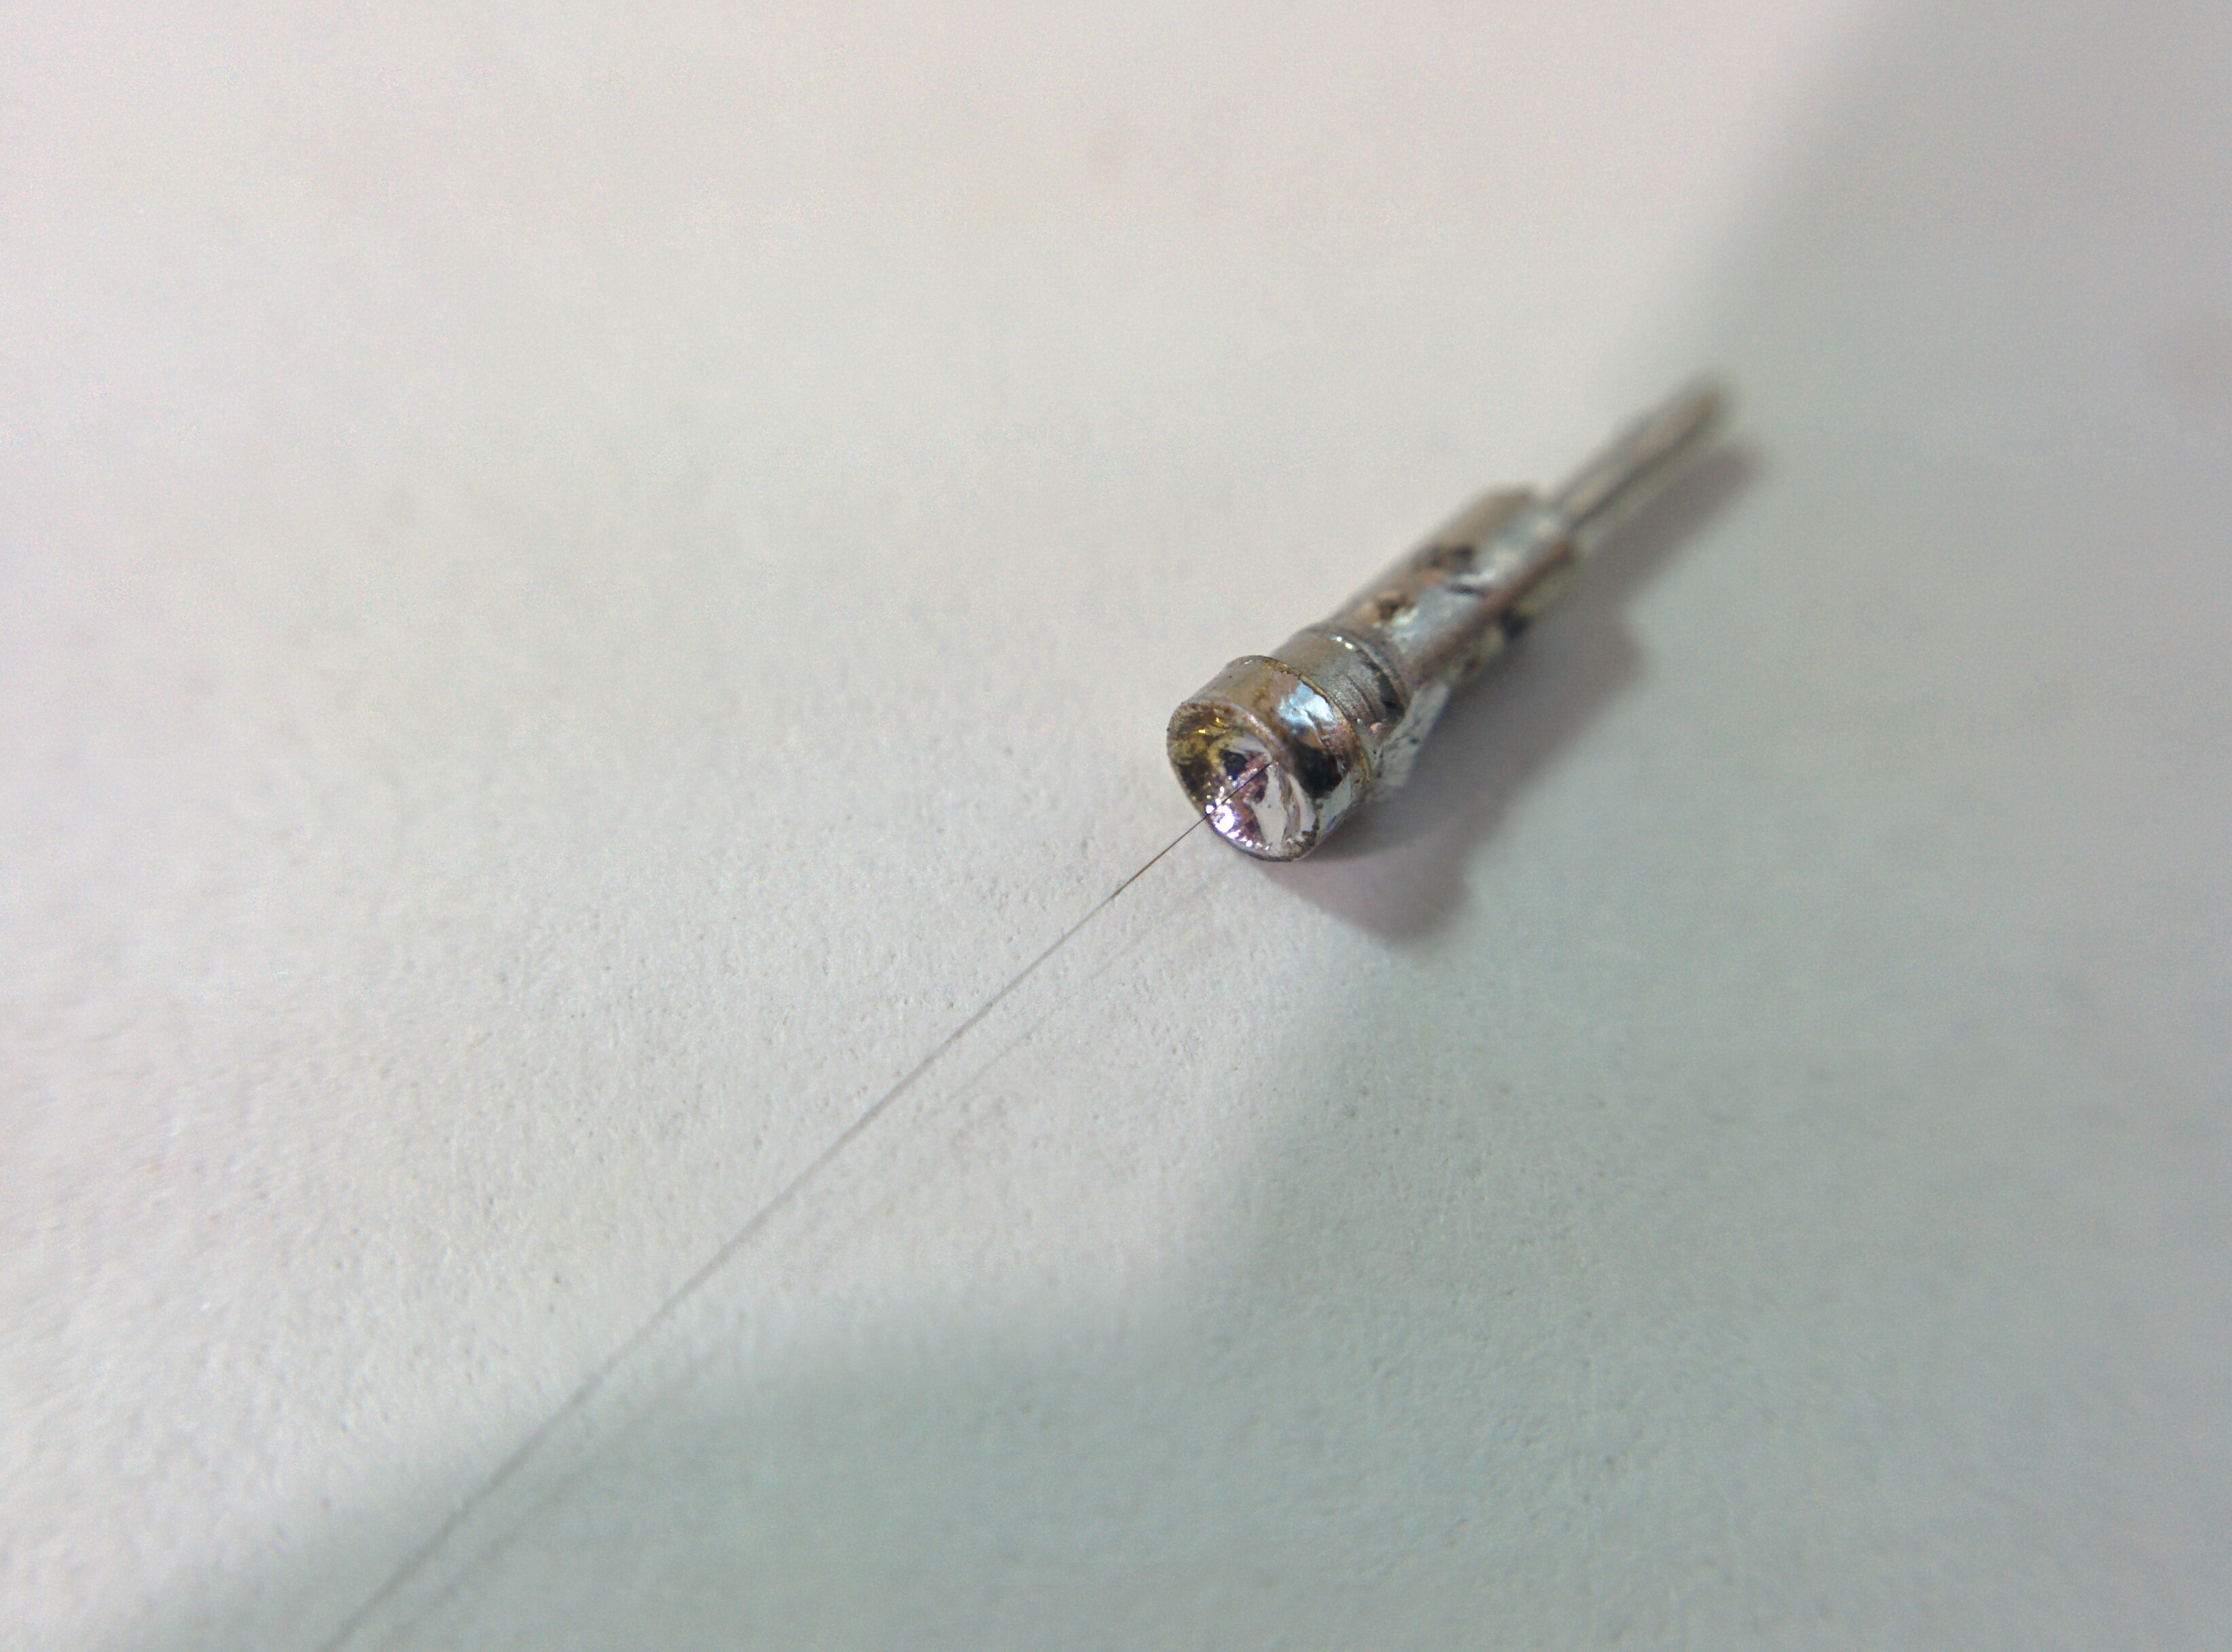
\includegraphics[trim = 10mm 20mm 0mm 10mm, clip, width=\s\textwidth]{microelectrode.jpg}
%\caption{}
%\label{fig:2d}
%\end{figure}

\def\s{0.15}
\def\left{70}
\def\bottom{120}
\def\right{50}
\def\top{30}
\begin{figure}
\centering
\begin{tikzpicture}
    \draw (0, 0) node[inner sep=0] {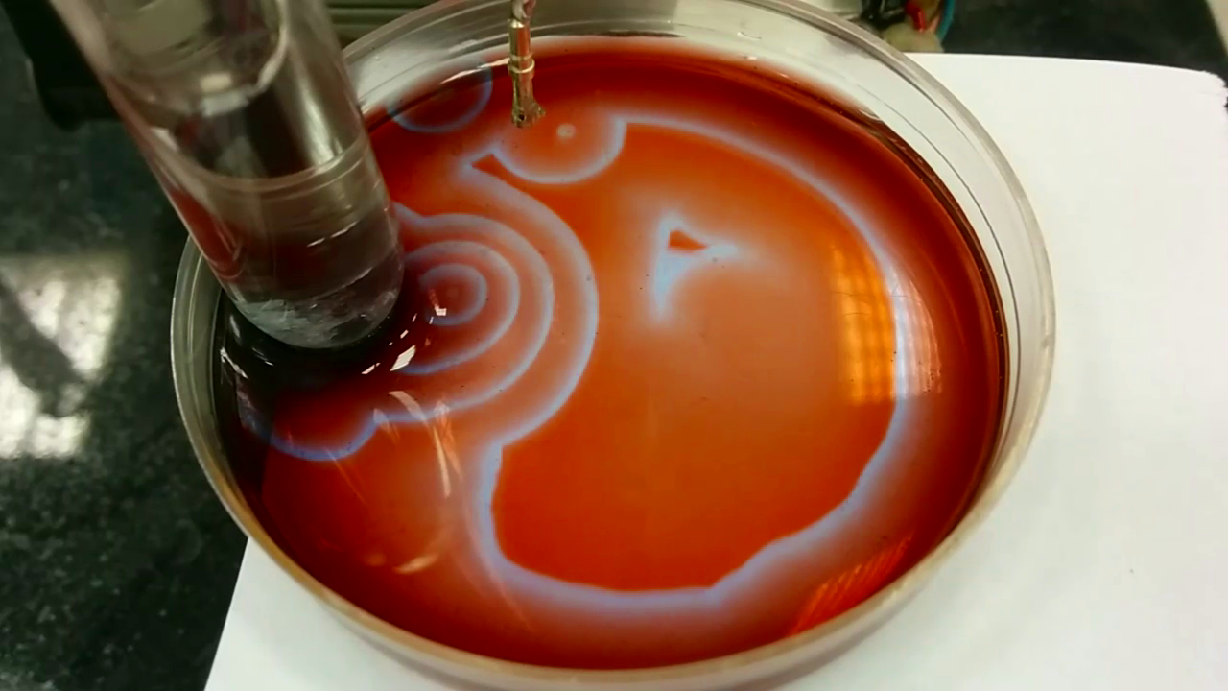
\includegraphics[trim = \left mm \bottom mm \right mm \top mm, clip, width=\s\textwidth]{0.png}};
    \draw (3.8, 1) node {a};
\end{tikzpicture}
\begin{tikzpicture}
    \draw (0, 0) node[inner sep=0] {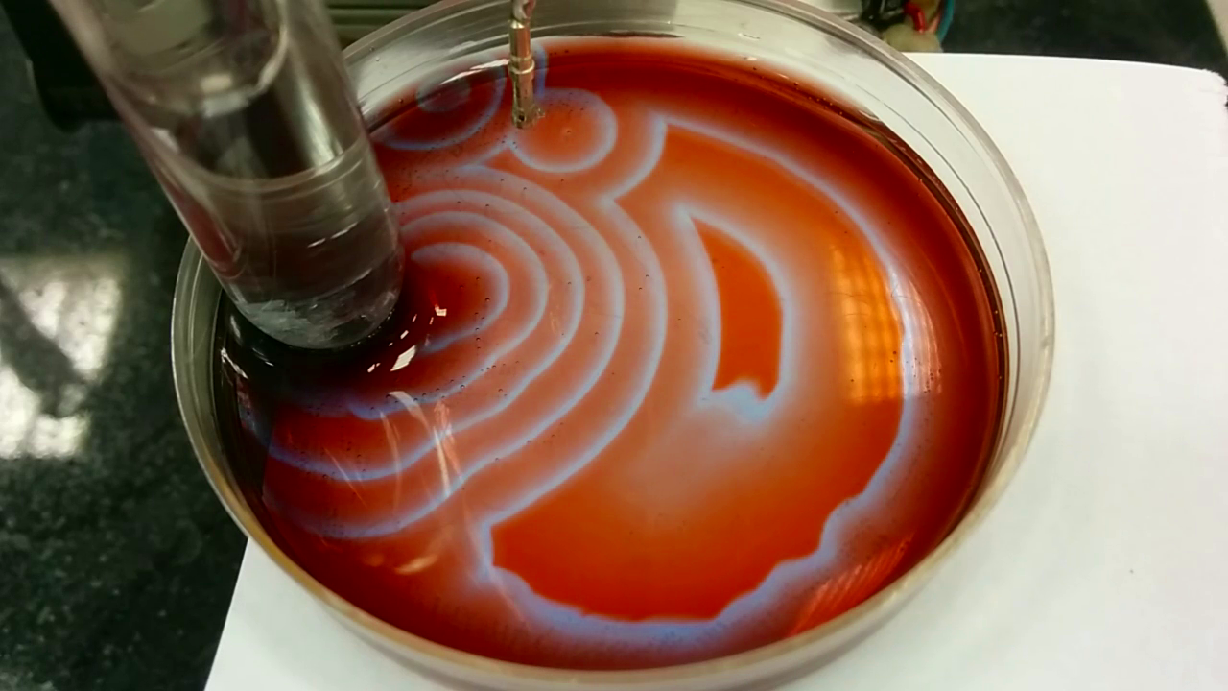
\includegraphics[trim = \left mm \bottom mm \right mm \top mm, clip, width=\s\textwidth]{1.png}};
    \draw (3.8, 1) node {b};
\end{tikzpicture}
\begin{tikzpicture}
    \draw (0, 0) node[inner sep=0] {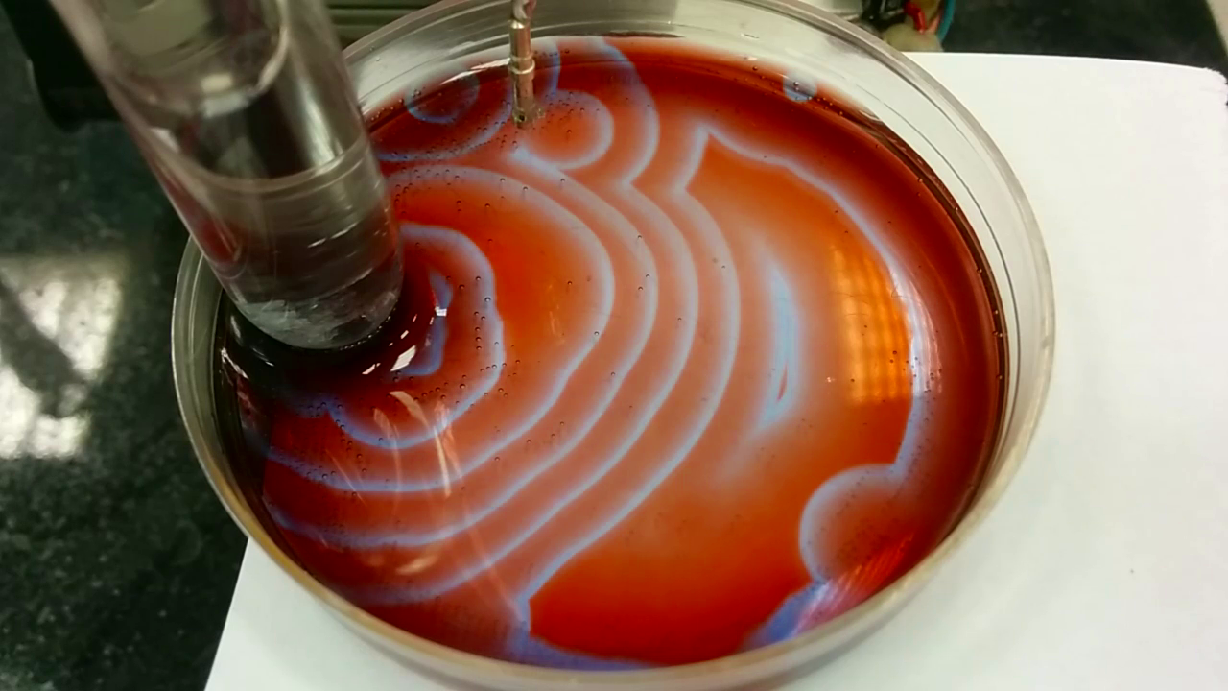
\includegraphics[trim = \left mm \bottom mm \right mm \top mm, clip, width=\s\textwidth]{2.png}};
    \draw (3.8, 1) node {c};
\end{tikzpicture}
\begin{tikzpicture}
    \draw (0, 0) node[inner sep=0] {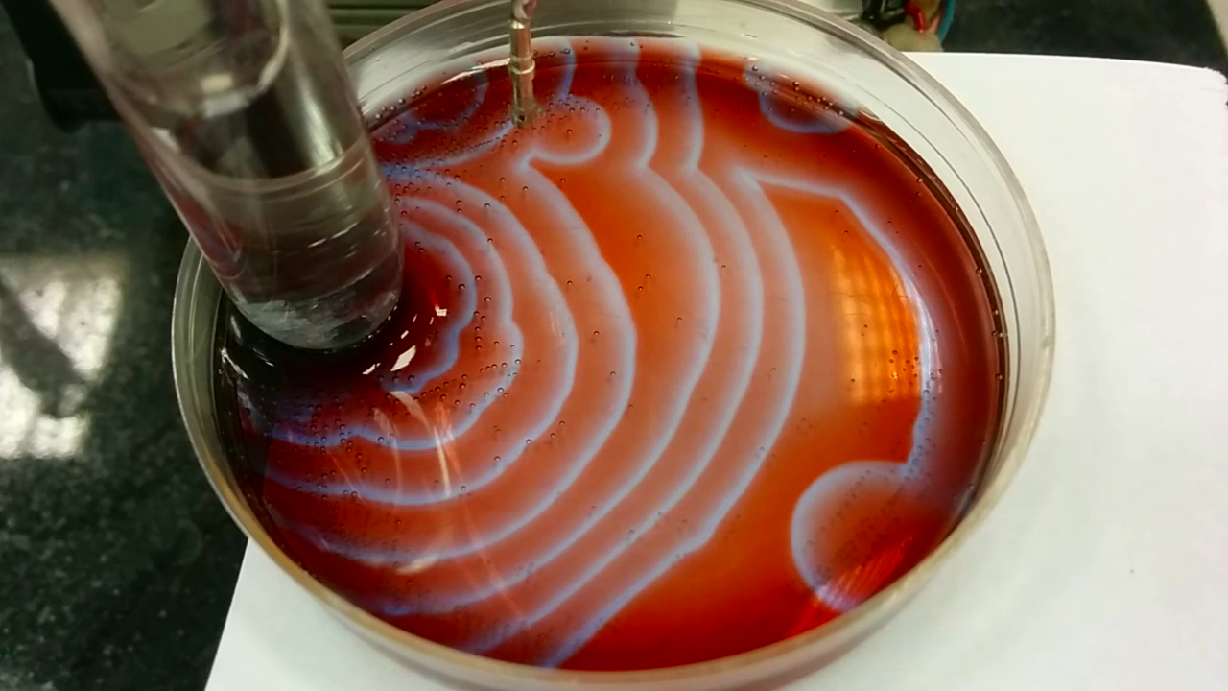
\includegraphics[trim = \left mm \bottom mm \right mm \top mm, clip, width=\s\textwidth]{3.png}};
    \draw (3.8, 1) node {d};
\end{tikzpicture}
\caption{}
\label{fig:2d}
\end{figure}

%\begin{tikzpicture}
%  \begin{axis}
%    \addplot3[colormap/viridis, surf, very thick] table {17101308_st_lines.txt};
%    %\addplot3[color=black, surf, very thick] table {17101308_st_lines.txt};
%  \end{axis}
%\end{tikzpicture}


\section{Conclusions}

\section*{References}

\begin{thebibliography}{5}

\end{thebibliography}

\end{document}
